
倍增法,通过字面意思来看就是翻倍。这个方法在很多算法中均有应用。其中最常用的就是 RMQ 问题和求 LCA 了。

\subsection{RMQ 问题}

\subsubsection{简介}

RMQ 是英文 Range Maximum / Minimum Query 的缩写,表示区间最大(最小)值。

解决 RMQ 问题的主要方法有两种,分别是 ST 表和线段树。本文主要讲 ST 表。

\subsubsection{引入}

\href{https://www.luogu.org/problemnew/show/P3865}{ST 表模板题}

题目大意:给定 $n$ 个数,有 $m$ 个询问,对于每个询问,你需要回答区间 $[x,y]$ 中的最大值

考虑暴力做法。每次都对区间 $[x,y]$ 扫描一遍,求出最大值

显然,这个算法会超时

\subsubsection{ST 表}

$ST$ 表基于倍增思想,可以做到 $O(n\log n)$ 预处理,$O(1)$ 回答每个询问。但是不支持修改操作。

暴力跑的慢的原因在于检索了每一个点。

但是,如果我们预处理出每一段的最大值,就可以将效率提高很多。

令 $f[i][j]$ 表示 $[i,i+2^j-1]$ 的最大值。

显然,$f[i][0]=a[i]$

根据定义式,写出状态转移方程:$f[i][j]=\max(f[i][j-1],f[i+2^{j-1}][j-1])$

我们可以这么理解:将区间 $[i,i+2^j-1]$ 分成相同的两部分

中点即为 $(i+(i+2^j-1))/2=i+2^{j-1}-1/2$

所以 $[i,i+2^j-1]$ 可以分成 $[i,i+2^{j-1}-1]$ 和 $[i+2^{j-1}+1,i+2^j-1]$

\begin{figure}[htbp]
\centering
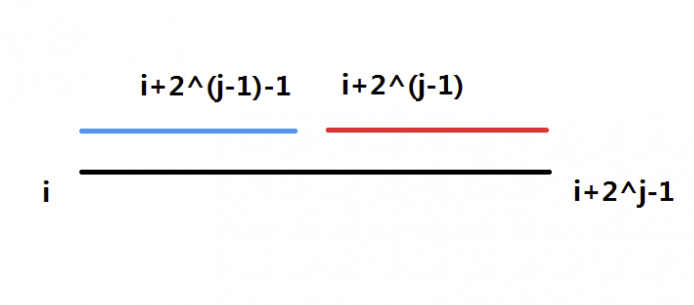
\includegraphics[width=0.7\textwidth]{docs/ds/images/st1.png} 

\end{figure}

预处理终于完成了!接下来就是查询了

对于每个询问 $[x,y]$,我们把它分成两部分

$f[x][s]$  $f[y-2^s+1][s]$

其中 $s=\log_2{(y-x+1)}$

显然,这两个区间会重叠。但是,重叠并不会对区间最大值产生影响。同时这两个区间刚好覆盖了 $[x,y]$,可以保证答案的正确性。

\subsubsection{模板代码}

\href{https://www.luogu.org/problemnew/show/P3865}{ST 表模板题}

\begin{cppcode}
#include <bits/stdc++.h>
using namespace std;
const int logn = 21;
const int maxn = 2000001;
long long a[maxn], f[maxn][logn], Logn[maxn];
inline int read() {
  char c = getchar();
  int x = 0, f = 1;
  while (c < '0' || c > '9') {
    if (c == '-') f = -1;
    c = getchar();
  }
  while (c >= '0' && c <= '9') {
    x = x * 10 + c - '0';
    c = getchar();
  }
  return x * f;
}
void pre() {
  Logn[1] = 0;
  Logn[2] = 1;
  for (int i = 3; i <= maxn; i++) {
    Logn[i] = Logn[i / 2] + 1;
  }
}
int main() {
  int n = read(), m = read();
  for (int i = 1; i <= m; i++) f[i][0] = read();
  pre();
  for (int j = 1; j <= logn; j++)
    for (int i = 1; i + (1 << j) - 1 <= n; i++)
      f[i][j] = max(f[i][j - 1], f[i + (1 << (j - 1))][j - 1]);
  for (int i = 1; i <= m; i++) {
    int x = read(), y = read();
    int s = Logn[y - x + 1];
    printf("%d\n", max(f[x][s], f[y - (1 << s) + 1][s]));
  }
  return 0;
}
\end{cppcode}

\subsubsection{注意点}

\begin{enumerate}
\item 输入输出数据一般很多,建议开启输入输出优化
\item 每次用 \href{https://en.cppreference.com/w/cpp/numeric/math/log}{std::log} 重新计算 log 函数值并不值得,建议如下预处理
\end{enumerate}

$$
\left\{\begin{aligned}
Logn[1] &=0, \\
Logn\left[i\right] &=Logn[\frac{i}{2}] + 1.
\end{aligned}\right.
$$

\subsubsection{总结}

$ST$ 表能较好的维护区间信息,时间复杂度较低,代码量相对其他算法不大。但是,$ST$ 表能维护的信息非常有限,不能较好地扩展,并且不支持修改操作。

\subsection{树上倍增求 LCA}

\subsubsection{LCA 简介}

LCA(Least Common Ancestors)表示最近公共祖先。

对于一棵有根树,设 $LCA(u,v)=x$,则 $x$ 必须满足以下条件

\begin{itemize}
\item $x$ 是 u 的祖先或 u
\item $x$ 是 v 的祖先或 v
\item $x$ 是在满足上面两个条件下深度最大的
\end{itemize}

显然,在一棵有根树内,对于任意两个节点有且仅有一个 $LCA$

解决这个问题,我们通常有以下方法

\begin{itemize}
\item 树上倍增(本文主要讲解此方法)
\item 转化为 RMQ 问题
\item 树链剖分
\item Tarjan
\end{itemize}

\subsubsection{暴力做法}

\begin{enumerate}
\item 将两个点跳到同一深度
将深度大的点 \textbf{ 一步一步 } 往上跳,发现另一个点是他的祖先,则另一个点就是 $LCA$
\item 一起往上跳
当两个点深度一样但是还没有找到 LCA 的时候,就一起往 \textbf{ 一步一步 } 上跳,知道跳到了同一个点。那么,这个点即为它们的 LCA
\end{enumerate}

\subsubsection{树上倍增}

暴力慢的原因在于跳的时候是 \textbf{ 一步一步 } 跳的,导致效率较低。如果我们可以 \textbf{ 一次跳多步 },效率就大大提高了。

\paragraph{预处理}

令 $f[i][j]$ 表示 $i$ 的 $2^j$ 辈祖先,及从 $i$ 向根节点走 $2^j$ 步到达的节点。$f[i][0]$ 就表示 $i$ 的父节点。

通过 $2^{j-1}\times 2^{j-1}=2^j$ 可以得到状态转移方程 $f[i][j]=f[f[i][j-1]][j-1]$\sout{(是不是和 $ST$ 的转移方程有点像)}。自然,当 $i$ 没有 $2^j$ 辈祖先时 $f[i][j]=0$

一遍 DFS 计算即可

\begin{cppcode}
void dfs(int u, int father) {
  dep[u] = dep[father] + 1;  // dep[x] 表示 x 的深度,在查询时会用到
  for (int i = 0; i <= 19; i++) f[u][i + 1] = f[f[u][i]][i];  // 预处理
  for (int i = first[u]; i; i = next[i])                      // 链式前向星
  {
    int v = go[i];
    if (v == father) continue;
    f[v][0] = u;  // f[v][0] 表示 v 的父亲
    dfs(v, u);
  }
}
\end{cppcode}

\paragraph{查询}

依然采用暴力的思想。先将两个节点跳到同一深度,然后一起往上跳。

只不过在跳的过程中从一步一步跳变成了 \textbf{ 一次跳多步 }。可以具体分为以下几步

\begin{enumerate}
\item 让 $x$ 的深度比 $y$ 大(深度在预处理时已经求出)
\item 将两个节点跳到同一深度。在此处我们使用二进制思想,依次尝试向上跳 $2^i,2^{i-1}\cdots 2^1,2^0$。如果发现则 $x$ 跳到了 $y$ 就说明 $LCA(x,y)=y$
\item 一起往上跳。依然使用二进制思想,让他们一起往上跳 $2^i,2^{i-1}\cdots 2^1,2^0$. 如果 $f[x][i]!=f[y][i]$,说明 $x$ 和 $y$ 还未相遇。最后,$x$ 和 $y$ 必定只差一步相遇。这时 $x$ 的父亲即 $f[x][0]$ 就是他们的 LCA
\end{enumerate}

\begin{cppcode}
int lca(int x, int y) {
  if (dep[x] < dep[y]) swap(x, y);  // 步骤 1
  for (int i = 20; i >= 0; i--)     // 步骤 2
  {
    if (dep[f[x][i]] >= dep[y]) x = f[x][i];
    if (x == y) return x;
  }
  for (int i = 20; i >= 0; i--)  // 步骤 3
    if (f[x][i] != f[y][i]) {
      x = f[x][i];
      y = f[y][i];
    }
  return f[x][0];
}
\end{cppcode}

\subsubsection{总结}

树上倍增法可以在 $O(n\log n)$ 的时间内完成预处理,在 $O(\log n)$ 的时间里完成查询,是一个较高效的算法,代码量也不大,一般竞赛推荐使用。

\subsection{练习}

\href{https://www.luogu.org/problemnew/show/P3865}{RMQ 模板题}

\href{https://www.luogu.org/problemnew/show/P3379}{LCA 模板题}

\href{https://www.luogu.org/problemnew/show/P4180}{严格次小生成树}

\href{https://www.luogu.org/problemnew/show/P1967}{货车运输}

\href{https://www.luogu.org/problemnew/show/P1613}{跑路}
